%%%%%%%%%%%%%%%%%%%%%%%%%%%%%%%%%%%%%%%%%
% Friggeri Resume/CV
% XeLaTeX Template
% Version 1.0 (5/5/13)
%
% This template has been downloaded from:
% http://www.LaTeXTemplates.com
%
% Original author:
% Adrien Friggeri (adrien@friggeri.net)
% https://github.com/afriggeri/CV
%
% License:
% CC BY-NC-SA 3.0 (http://creativecommons.org/licenses/by-nc-sa/3.0/)
%
% Important notes !!! : 
% Use texshop for better editor and this template needs to be compiled with XeLaTeX and the bibliography, if used,
% needs to be compiled with bibtex with biber backend.
%
%%%%%%%%%%%%%%%%%%%%%%%%%%%%%%%%%%%%%%%%%

\documentclass[style=verbose,maxnames=99,sorting=ydnt,backend=biber]{friggeri-cv} % Add 'print' as an option into the square bracket to remove colors from this template for printing

\addbibresource{cv-dhoto-kavli2016.bib} % Specify the bibliography file to include publications
%\usepackage[backend=biber]{biblatex}


\usepackage{wrapfig}



\begin{document}

\header{Sritrusta}{ Sukaridhoto}{Assistant Prof., Researcher and Guitarist} % Your name and current job title/field

%----------------------------------------------------------------------------------------
%	SIDEBAR SECTION
%----------------------------------------------------------------------------------------

\begin{aside} % In the aside, each new line forces a line break
\section{contact}
\textbf{Politeknik Elektronika Negeri Surabaya}
Jl. Raya ITS Surabaya
~
Office:+62 (31) 5947280
Mobile:+62 823 6666 6379
~
\href{mailto:dhoto@pens.ac.id}{dhoto@pens.ac.id}
\href{http://dhoto.lecturer.pens.ac.id/}{Dhoto's Homepage}
\href{http://facebook.com/iseng4h}{fb://iseng4h}
\section{languages}
Indonesian (native)
English \& Japanese 
\section{research interests}
{\color{red} $\varheartsuit$} Computer Networks,
Embedded System, Multimedia \& Internet of Things
\end{aside}

%----------------------------------------------------------------------------------------
%	EDUCATION SECTION
%----------------------------------------------------------------------------------------

\section{biography}

\begin{wrapfigure}[20]{l}{1.5in}
	\vspace{-10pt}
	\begin{center}
    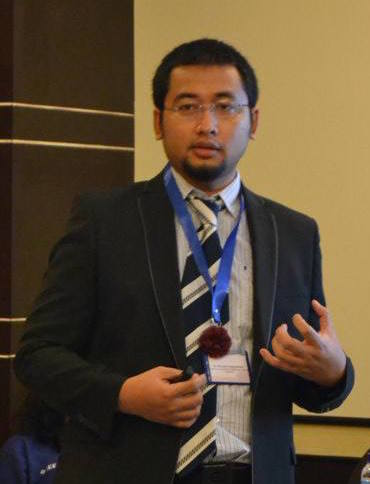
\includegraphics[width=0.2\textwidth]{dhoto-jas.jpg}
    \end{center}
    
\end{wrapfigure}
Received the B.E. degree in electrical engineering, computer science program from Sepuluh Nopember Institute of Technology, Indonesia, in 2002 and the Ph.D. degree in Communication Networks Engineering from Okayama University, Japan, in 2013. He joined at Electronics Engineering Polytechnic Institute of Surabaya, Indonesia, as a lecturer in 2002. He stayed at Tohoku University, Japan, in 2004, as a visiting researcher. His research interests include computer networks, embedded system, multimedia and Internet of Things. He received IEEE Young Researcher Award in 2009. He is a member of IEEE.



\section{education}

\begin{entrylist}
%------------------------------------------------
\entry
{2009--2013}
{Doctor {\normalfont of Philosophy}}
{Okayama University, Japan}
{\emph{Engineering} \\ 
Dissertation: "A Study of Performance Improvement Methods for Real-Time Applications in Wireless Mesh Networks" \\
Supervised by Prof. Nobuo Funabiki, Prof. M. Hata and Prof. Toru Nakanishi}
%------------------------------------------------
\entry
{1997--2002}
{Bachelor {\normalfont of Engineering}}
{Institut Teknologi Sepuluh Nopember, Indonesia}
{Electrical Engineering - Computer Science\\
Thesis: “Implementation of IPv6 at Institute Technology Sepuluh November of Surabaya” 
\\Supervised by Dr. Surya Sumpeno and Dr. Supeno Mardi
}

%------------------------------------------------
\end{entrylist}

%----------------------------------------------------------------------------------------
%	WORK EXPERIENCE SECTION
%----------------------------------------------------------------------------------------

\section{work experience}

\begin{entrylist}
%------------------------------------------------
\entry
{2002-Now}
{Politeknik Elektronika Negeri Surabaya}
{Surabaya, Indonesia}
{\emph{Assistant Professor} \\
Department of Multimedia Creative Technology, 
\begin{itemize}
\item Teaching : Data Communication and Computer Networks
\item Supervision of Diploma students
\end{itemize}
Graduate School of Information Technology, 
\begin{itemize}
\item Teaching : Advanced Computer Networks and Internet of Things
\item Supervision of Master students
\end{itemize}
}

\end{entrylist}
\\
\\



%----------------------------------------------------------------------------------------
%	AWARDS SECTION
%----------------------------------------------------------------------------------------

\section{award}
\begin{entrylist}
%------------------------------------------------
\entry
{2014}
{Best Paper Award}
{The 16th International Electronics Symposium, Indonesia}
{\emph{Application Programming Interface Design of Microkernel Based Robotics Operating System}, Adhe Widianjaya, Dadet Pramadihanto, Sritrusta Sukaridhoto; The 16th International Electronics Symposium, Indonesia}


%------------
\entry
{2009}
{IEEE’s Young Researcher Award}
{ISCE2009, Japan}
{}
%------------------------------------------------
%\entry
%{2009}
%{Monbusho Scholarship for Doctoral Program}
%{Okayama University, Japan}
%{}
%------------------------------------------------

\end{entrylist}

%---------------------
%Research Grant
%--------------------

\section{research grants}

\begin{entrylist}


\entry
{2016}
{DESIGN AND DEVELOPMENT OF UNMANNED UNDERWATER VEHICLES FOR ENVIRONMENTAL MONITORING AND DATA ACQUISITION COMPATIBLE WITH 5D WORLD MAP SYSTEM IN INTERNET OF UNDERWATER THINGS}
{DIKTI}
{Penelitian Kerjasama Luar Negeri dan Publikasi International - year: 2 of 3 - Rp. 160.000.000,-}

\entry
{2016}
{Pusat Pendidikan dan Pelatihan Embedded System Bersertifikasi Sebagai Upaya Penyiapan Sumber Daya Manusia Menjelang Masyarakat Ekonomi ASEAN}
{DIKTI}
{Ipteks Bagi Inovasi Kreativitas Kampus - year: 1 of 3 - Rp. 189.000.000,- + Rp 50.000.000,-}


\entry
{2015}
{DESIGN AND DEVELOPMENT OF UNMANNED UNDERWATER VEHICLES FOR ENVIRONMENTAL MONITORING AND DATA ACQUISITION COMPATIBLE WITH 5D WORLD MAP SYSTEM IN INTERNET OF UNDERWATER THINGS}
{DIKTI}
{Penelitian Kerjasama Luar Negeri dan Publikasi International - year: 1 of 3 - Rp. 157.500.000,-}


\end{entrylist}


%----------------------------------------------------------------------------------------
%	PUBLICATIONS SECTION
%----------------------------------------------------------------------------------------



\section{publications}




\nocite{*}

\printbibsection{article}{Journals} % Print all articles from the bibliography

%\begin{refsection} % This is a custom heading for those references marked as "inproceedings" but not containing "keyword=france"
%\newrefcontext[sorting=ydnt]
\printbibliography[type=inproceedings, title={Conferences/Proceedings}, heading=subbibliography]
%\end{refsection}

%\printbibsection{book}{Books} % Print all books from the bibliography

%----------------------------------------------------------------------------------------

\section{signature}

The fully truth of the details are guaranteed. 
With strong sense of responsibility, hands on management and communication skills. 
Strong loyalty and self-motivation. 
\\
\\ 
regards, 
\\ 
\\
\\
\\
\textbf{Sritrusta Sukaridhoto, ST. Ph.D.} 


\end{document}